\begin{minipage}{0.55\textwidth}
    \begin{figure}[h]
    \centering
    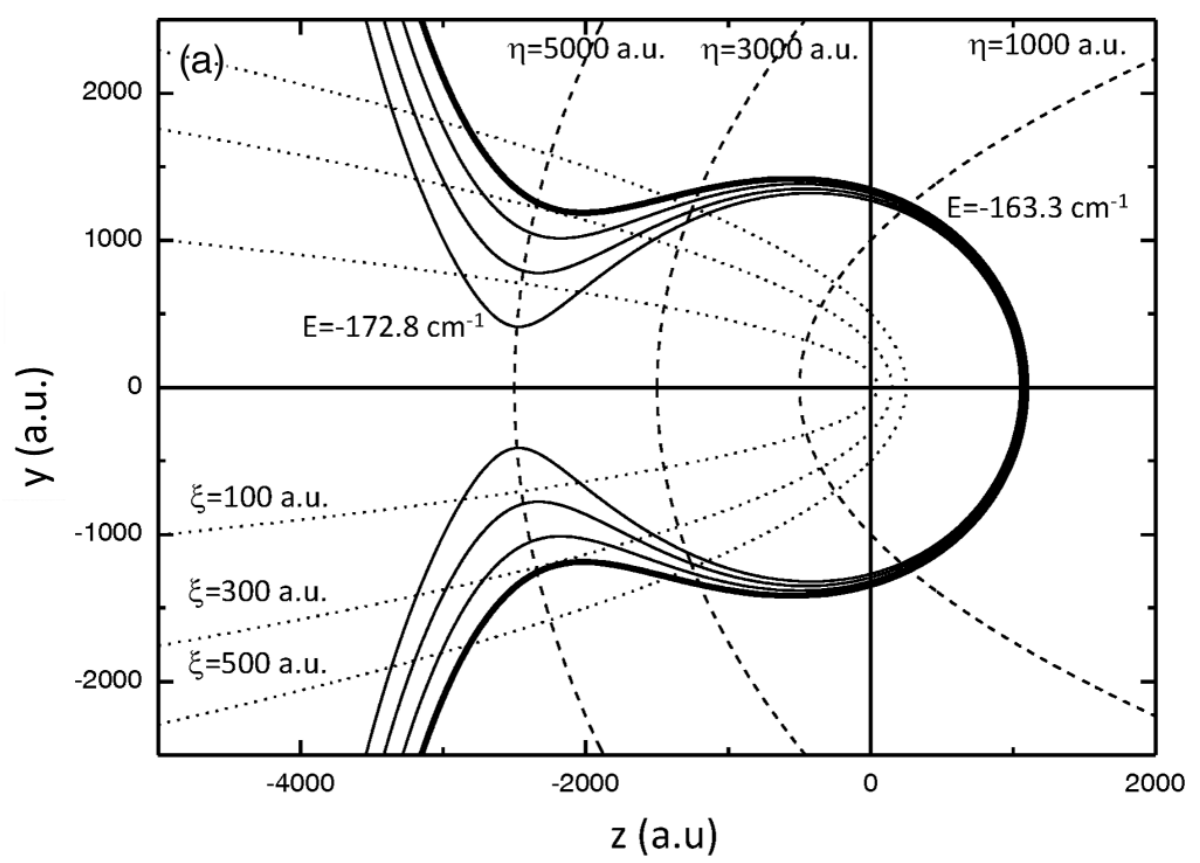
\includegraphics[width=1.1\textwidth]{figures/parabola.png}
    % \caption{}
    %\label{fig:}
\end{figure}
\end{minipage}
\hfill
\begin{minipage}{0.35\textwidth}
    % В статическом электрическом поле волновая функция водорода может быть разделена в смысле параболических координат
    For $z$ --- displacement along the electric field.
    And $r$ --- electron-proton distance.
    \begin{gather*}
    	\eta = r - z \\
    	\xi  = r + z 
    \end{gather*}
\end{minipage}
\begin{equation*}
	\Psi(\xi,\eta,\varphi) = \frac{1}{\sqrt{2 \pi \eta \xi}} \chi_1(\xi) \chi_2(\eta) e^{i m \varphi}
\end{equation*}
